\documentclass[journal]{IEEEtran}

\usepackage[spanish]{babel}
\usepackage[utf8]{inputenc}
\usepackage[T1]{fontenc}
\usepackage{graphicx}
\usepackage{amssymb}
\usepackage{amsmath}
\usepackage{amsthm}
\usepackage{booktabs}
\usepackage{gensymb}
\usepackage{stfloats}
\usepackage{float}
\usepackage{nccmath}
\usepackage{caption}
\usepackage{url}
\usepackage{listings}

\title{\textbf{SSH y STP}}

\author{Redes LAN/WAN \\
	\textit{Profesor:} Luis Fernando Díaz Cadavid - Jaime Alberto Sepúulveda\\
	\textit{Monitores:} Juan José Jaramillo Granada - 814034 \\
	Kevin Leonardo Cerpa Campanella - 814017 \\
	Universidad Nacional de Colombia - Sede Manizales}

\date{}

\begin{document}
\maketitle

\section{\textbf{Descripción.}}
En esta práctica se introducirán los conocimientos necesarios para configurar un Switch con los protocolos SSH y STP en las plataformas de simulación de cisco y Huawei, e introducir conceptos como puertos troncales y  enlaces de agregación.

\section{\textbf{protocolo SSH}}
El protocolo SSH (también conocido como Secure Shell) es un método para el inicio de sesión remoto seguro desde una computadora a otra. Ofrece varias opciones alternativas para una autenticación fuerte y protege la seguridad e integridad de las comunicaciones con un cifrado sólido. Es una alternativa segura a los protocolos de inicio de sesión no protegidos (como telnet , rlogin) y métodos de transferencia de archivos inseguros (como FTP ).

\section{\textbf{Spanning tree o STP}}
Es un protocolo de red de capa 2 del modelo OSI (capa de enlace de datos). Su función es la de gestionar la presencia de bucles en topologías de red debido a la existencia de enlaces redundantes (necesarios en muchos casos para garantizar la disponibilidad de las conexiones). El protocolo permite a los dispositivos de interconexión activar o desactivar automáticamente los enlaces de conexión, de forma que se garantice la eliminación de bucles.

\begin{figure}[ht]
	\centering
	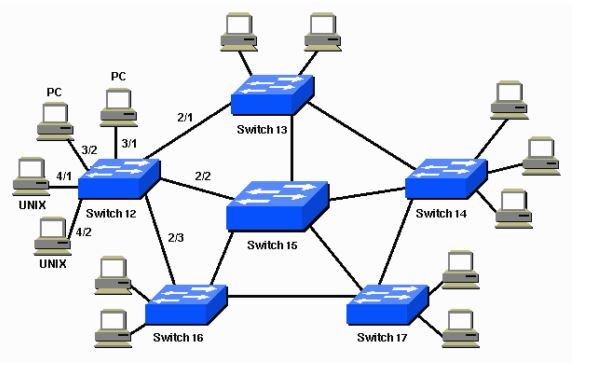
\includegraphics[scale=0.5]{2.jpg}
	\caption{Trunking}
\end{figure}

\section{\textbf{ Puertos Troncales(TRUNK)}} 
Trunk es una configuración de canal para puertos de switch que estén en una red Ethernet, que posibilita que se pueda pasar varias VLAN por un único link, o sea, un link de troncal es un canal que puede ser switch-switch o switch-router, por donde se pasan informaciones originadas y con destino a más de una VLAN.; así el link de la troncal no pertenece a ninguna VLAN individualmente.

\section{\textbf{agregación de enlaces o Trunking}}
La agregación de enlaces, o IEEE 802.3ad, es un término que indica el establecimiento de una red de datos que describe cómo utilizar varios enlaces Ethernet full-dúplex en la comunicación entre dos equipos, repartiendo el tráfico entre ellos,  es una manera económica de instalar una red de alta velocidad más rápida de lo que permita un solo puerto o dispositivo de la tecnología de que se disponga. Básicamente consiste en agrupar varios dispositivos que trabajan simultáneamente a su velocidad máxima como si fuera un único enlace de mayor capacidad.

\begin{figure}[ht]
	\centering
	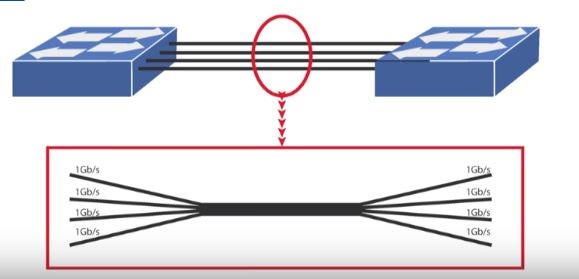
\includegraphics[scale=0.5]{1.jpg}
	\caption{Trunking}
\end{figure}

\section{\textbf{Configuración de protocolo SSH en eNSP}}
Montamos la siguiente topologia:

\begin{figure}[ht]
	\centering
	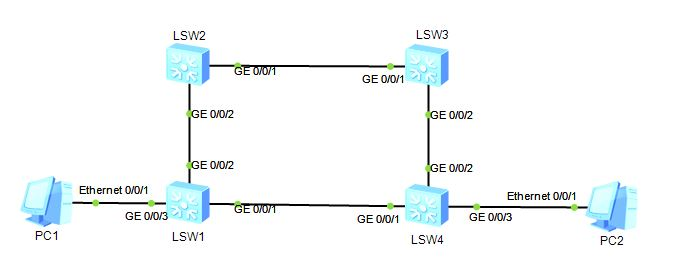
\includegraphics[scale=0.5]{4.jpg}
	\caption{Topologia STP}
\end{figure}

Antes de configurar las funciones básicas de STP / RSTP, debe configurar el modo de trabajo de un dispositivo de conmutación a STP / RSTP.

\begin{enumerate}
	\item \textbf{Escoger el switch root}\\
	
	Cuanto más bajo es el valor numérico, más alta es la prioridad que tiene un dispositivo de conmutación y más probable es que se seleccione el dispositivo de conmutación como puente raíz.\\
	
	\textit{Nota: El valor de prioridad predeterminado de un dispositivo de conmutación es 32768.}
	
	\begin{lstlisting}[frame=single]
system-view
		\end{lstlisting}
		\begin{lstlisting}[frame=single]
stp mode { stp | rstp }
		\end{lstlisting}
		
		\begin{lstlisting}[frame=single]
stp priority 4096
		\end{lstlisting}

	\item Daremos valores de costo a cada puerto utilizado en cada switch de tal forma que queden como en la figura
	
	\begin{figure}[ht]
		\centering
		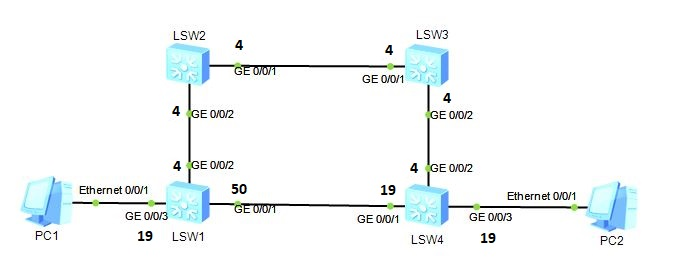
\includegraphics[scale=0.5]{5.jpg}
	\end{figure}

	\begin{lstlisting}[frame=single]
system-view
		\end{lstlisting}
	\begin{lstlisting}[frame=single]
stp mode stp
		\end{lstlisting}
		\begin{lstlisting}[frame=single]
interface GigabitEthernet 0/0/x
		\end{lstlisting}
		\begin{lstlisting}[frame=single]
stp cost 4 19  50
		\end{lstlisting}
		
	\item Asignamos IP y máscara correspondiente a cada PC
	
	\begin{figure}[ht]
		\centering
		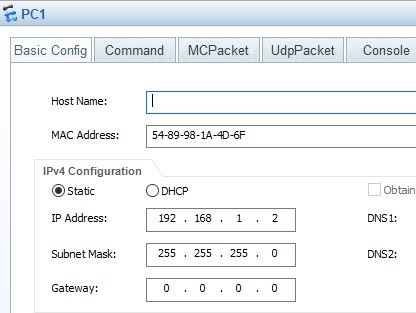
\includegraphics[scale=0.6]{7.jpg}
	\end{figure}

	\item Entramos al CLI del pc y enviamos un ping del PC1 al PC2 y comprobamos que el ping llegue.
	
	\newpage
	
	\begin{figure}[ht]
		\centering
		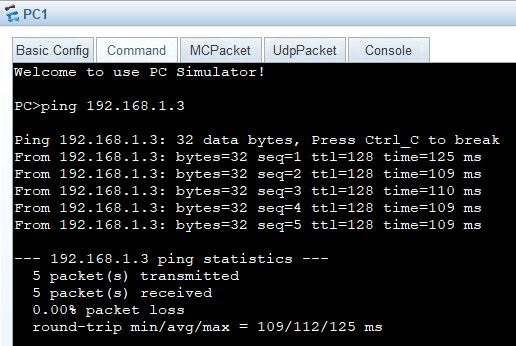
\includegraphics[scale=0.6]{8.jpg}
	\end{figure}

	\item Eliminamos la conexión entre switch 2 y switch 3 para simular un daño en el canal.
	
	\begin{figure}[ht]
		\centering
		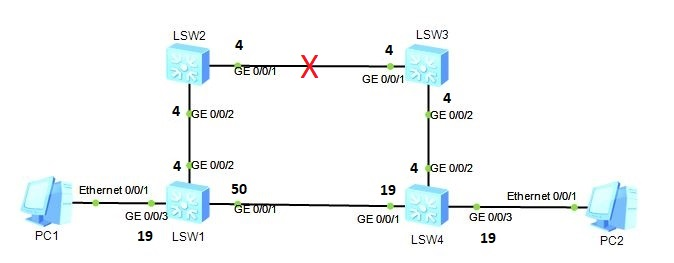
\includegraphics[scale=0.55]{6.jpg}
	\end{figure}

	\item Volvemos al CLI del pc y comprobamos que el ping se envía por el canal que queda activo
\end{enumerate}

\end{document}